\chapter{Universal Constructions I}
We've been hinting at the utility of knowing that categories that have certain
special objects in them. For example, if we want to give a category that lets us
validate equations of programming languages, that category will need to be able 
to represent the many features that programs might have: products, sums, 
functions, etc. Here we will introduce the essential idea of a \textbf{universal 
construction} that characterizes when categories contain these special objects.

\section{Terminal objects \& the unit type}
Recall that when designing categorical semantics for programming languages we
associate types and typing contexts with objects in the category and terms with
morphisms. Concretely, if we have a well-typed term $\Gamma \vdash e : A$,
its interpretation $\dbracket{\Gamma \vdash e : A}$ is a morphism
$\dbracket{\Gamma} \xrightarrow{\dbracket{e}} \dbracket{A}$.
Previously, we showed how \(\FinSet\) can be used to give an interpretation 
to \ref{lang:calc} programs by associating types like the unit type $\plUnit$
with special sets, like a set containing only a single element $\{\star\}$.
But, what if we want to see if categories other than $\FinSet$ can give give a 
reasonable interpretation for $\plUnit$?

To proceed, let's pick a particular object $\dbracket{\plUnit}$ 
in a category $\calC$ and explore what properties it needs to have in order 
to be ``$\plUnit$-like'':
\begin{itemize}
  \item \textbf{Fact 1, Introduction rules}: It must be possible in any typing context to
  produce a value of type $\plUnit$.  This tells us that for any context
  $\Gamma$, there must exist a $\calC$-morphism
  $\dbracket{\Gamma} \to \dbracket{\plUnit}$.
  For example, it must 
  be the case that 
  $\dbracket{\Gamma} \xrightarrow{\dbracket{\plunit}} \dbracket{\plUnit}$.

  \item \textbf{Fact 2, Equational laws}: Since \ref{lang:calc} has no effects, 
  it is the case that if $\Gamma \vdash e : \plUnit$, then it is indistinguishable 
  from the term $\plunit$. This is called \textbf{eta equality}, and we write
  this as $e \equiv \plunit$.\footnote{The symbol ``$\equiv$'' means ``is
  equationally equal to''.} Eta equality is an equational law that characterizes
  how a $\plUnit$ term must behave. Now for an insight: \emph{these equational
  laws are translated into morphism equalities}. It must be that, for any
  morphism $\dbracket{\Gamma} \xrightarrow{\dbracket{e}} \dbracket{\plUnit}$, it
  is the case that $\dbracket{e} = \dbracket{\plunit}$.  In other words, the
  morphism $\dbracket{\Gamma} \xrightarrow{\dbracket{\plunit}} \plUnit$ must be
  unique.
\end{itemize}

These two properties can be packaged up into a nice concise definition:

\begin{definition}[Terminal object] 
  Let $T$ be an object in a category $\calC$. 
  An object $T$ in $\calC$ is called a terminal object
  if, for every other object $A$ in $\calC$ there exists a unique 
  morphism $A \xrightarrow{\langle \rangle} T$. Graphically,

  \begin{center}
% https://tikzcd.yichuanshen.de/#N4Igdg9gJgpgziAXAbVABwnAlgFyxMJZABgBpiBdUkANwEMAbAVxiRAEEQBfU9TXfIRQBGclVqMWbACrdxMKAHN4RUADMAThAC2SMiBwQkokAyxhWiEHAhmoIagzoAjGAwAK-PATYMYanAcJZksQAB0wmAAPLDgcOABCOS4gA
\begin{tikzcd}
  A \arrow[r, "\exists!"] & T
  \end{tikzcd}
\end{center}
\end{definition}

Let's pause to remark on the three categorical interpretations 
of terminal objects $T$:
\begin{itemize}
  \item Graphically, an object is terminal if (1) there is an arrow from 
  every other object to it, and (2) it ``thins all parallel
  arrows'', meaning that if we have a situation like the following for 
  and morphisms $X \xrightarrow{f} T, X \xrightarrow{g} T$:
  \begin{align*}
    % https://tikzcd.yichuanshen.de/#N4Igdg9gJgpgziAXAbVABwnAlgFyxMJZABgBpiBdUkANwEMAbAVxiRABUQBfU9TXfIRRkAjFVqMWbABrdxMKAHN4RUADMAThAC2SEdRwQkZEACMYYKEgC0AZhMM65hgAV+eAmw1ZFACxwg1PTMrIggity8IJo6egZGiCbmlkj21I7ObtgeQiAMMGoBQZKh0XJcQA
\begin{tikzcd}
  T                                                       \\
  X \arrow[u, "g"', bend right] \arrow[u, "f", bend left]
  \end{tikzcd},
  \end{align*}
  then we know that $f = g$.
  \item The order-theoretic perspective is that the terminal object 
  is the ``greatest object'' in the category.
  \item The algebraic perspective yields the natural equations:
  for any morphism from $A \xrightarrow{f} T$, it is the case 
  that $f = \langle \rangle$.
\end{itemize}

We say a category \textbf{has terminal objects} if there is an object in the
category that is a terminal object. This is our first example of a 
\textbf{universal construction}, which are special objects in categories 
characterized by their morphisms into them. We will see how universal 
constructions can be used to give interpretations to all the type 
formers we have seen so far. But, we can already see their utility: 
whether or not a particular category admits certain universal constructions
will immediately inform us of that category's suitability for modeling 
certain language properties.

\subsection{$\FinSet$ has terminal objects, isomorphisms}
We saw in previous lectures that we could use the singleton set 
$\{\star\}$ to give an interpretation to $\plUnit$ in $\FinSet$.
We can easily prove that $\{\star\}$ is a terminal object:
\begin{theorem}
  The singleton set $\{\star\}$ is terminal in $\FinSet$.
\end{theorem}
\begin{proof}
  \begin{itemize}
    \item Existence: The map $\_ \mapsto \{\star\}$ has the required type.
    \item Uniqueness: Suppose we have two morphisms $A \xrightarrow{f} \{\star\}$ and
    $A \xrightarrow{g} \{\star\}$. 
    Then by function extensionality we immediately have that $f = g$ 
    as set-functions, and so they are equal as $\FinSet$ morphisms.
  \end{itemize}
\end{proof}

Now you can observe the above proof and see that it immediately 
works for \emph{any} choice of singleton set: does this mean that $\FinSet$
has \emph{many terminal objects?} Yes, and no. \emph{Yes}, in the sense 
that there are indeed many valid choices of terminal object; but \emph{no}, 
in the sense that the choice itself does not (\emph{should} not!) actually 
matter. We capture this by the notion of isomorphism:

\begin{definition}[Isomorphism of objects]
  \sloppy
  Two objects $A$ and $B$ in a category $\calC$ are isomorphic if 
  there exist morphisms $A \xrightarrow{f} B$ and $B \xrightarrow{g} A$
  such that (1) $g \circ f = \id_A$ and (2) $f \circ g = \id_B$.
\end{definition}

We can immediately see that any two singleton sets in $\FinSet$ are isomorphic:
this proof is straightforward. What might be surprising is that this 
fact is true for all terminal objects:

\begin{theorem} \label{thm:terminal-object-unique}
  Terminal objects are unique up to isomorphism.
\end{theorem}
\begin{proof}
  Let $X$ and $Y$ be terminal objects in some category $\calC$. 
  Then there exists a pair of unique morphisms between them:

  \begin{center}
 % https://tikzcd.yichuanshen.de/#N4Igdg9gJgpgziAXAbVABwnAlgFyxMJZABgBpiBdUkANwEMAbAVxiRAA0QBfU9TXfIRQBGclVqMWbAJrdxMKAHN4RUADMAThAC2SMiBwQkokACMYYKEgDM++s1aIQAQjXdeITTuPVDe6uaWNnaSji6KclxAA
\begin{tikzcd}
  X \arrow[r, "!f", bend left] & Y \arrow[l, "!g", bend left]
  \end{tikzcd} 
\end{center}
By the fact that $X$ and $Y$ are terminal, they must also have unique identity
morphisms $\id_X$ and $\id_Y$. Then by the uniqueness of identity we have that $f \circ g = \id_X$ and $g \circ f = \id_Y$.
\end{proof}

This provides some evidence that the choice of terminal object does not matter.
  But are we done? Suppose we had two terminal objects \(T\) and \(T'\).
  By the above argument, we have that these two objects are isomorphic.
  But now another potential choice arises: what if there are multiple different
  \emph{isomorphisms} between \(T\) and \(T'\)?
  Then it could be that the choice to use \(T\) instead of \(T'\)
  may implicitly come with a choice of specific isomorphism as well.

  Luckily, terminal objects satisfy a stronger property
  which ensures that one's choice is terminal object is truly irrelevant.

\begin{proposition}
  Terminal objects are unique up to \emph{unique} isomorphism.
  That is, if \(T\) and \(T'\) are both terminal,
  then there is exactly one isomorphism
  \((f:T\to T',g:T'\to T)\)
  between \(T\) and \(T'\).
\end{proposition}
\begin{proof}
  Both \(f\) and \(g\), as constructed in the proof of
  \Cref{thm:terminal-object-unique},
  are the only possible morphisms \(T \to T'\) and \(T'\to T\)
  respectively. Thus they together form the only isomorphism
  between \(T\) and \(T'\).
\end{proof}

Later on, when we have the language for it, we will show that
all universal constructions are unique up to unique isomorphism
in this sense, and hence free of non-canonical choices.

% \subsection{Terminal objects for preorders}
% Universal constructions are one of the engines for analogy in category theory:
% very different-seeming concepts can be cast as instances of the same 
% universal construction, which can bring clarity to what each of those disparate 
% concepts means. When cast order-theoretically, the terminal object can 
% be thought of as ``the greatest object in a category.''
% % The first instance we will see of a universal construction is a \textbf{terminal 
% % object}, which can be thought of as ``the largest object in a category'' if one 
% % recalls the preorder intuition of morphisms. 

% An element of a preorder is the largest if it is greater than every other 
% element: i.e., there exists a morphism from every other element to it.
% This definition works for a general category: one could say an object is 
% largest if there exists a morphism from every other object into it.
% This characterization however doesn't take into account that there 
% can be more than 1 morphism between any two objects in a category: intuitively, 
% this means that one object can be greater than another in more than one way.

\section{Products}
Next we want to interpret product types $A \times B$. As before with the 
unit type, the typing rules for products forces the existence of certain morphisms,
and the equational theory of products forces equalities of certain morphisms.
The  introduction rule that describes how to create new products is:
\begin{mathpar}
\inferrule
    {\Gamma\vdash M : A
      \\
    \Gamma\vdash N : B
    }
    {\Gamma \vdash \plpair{M}{N} : A \pltimes B}~(\textsc{T-Pair})
\end{mathpar}
The elimination rules that break apart products are:
\begin{mathpar}
\inferrule
    {\Gamma\vdash M : A \pltimes B}
    {\Gamma \vdash \plfst{M} : A}~(\textsc{T-Fst})
\and
\inferrule
    {\Gamma\vdash M : A \pltimes B}
    {\Gamma \vdash \plsnd{M} : B}~(\textsc{T-Snd})
\end{mathpar}

These rules imply the existence of several morphisms that characterize 
what it means for for a special object $\dbracket{A \times B}$ to be a 
product. Reading off from the rules:
\begin{itemize}
  \item The \textsc{T-Pair} rules says that if there are 
  two morphisms $\dbracket{\Gamma} \mor{\dbracket{M}} \dbracket{A}$ and 
  $\dbracket{\Gamma} \mor{\dbracket{N}} \dbracket{B}$, 
  then there is a morphism $\dbracket{\Gamma} \mor{\dbracket{\langle M, N \rangle}} 
  \dbracket{A \times B}$.
  \item The \textsc{T-Fst} rule says that if there is a morphism 
  $\dbracket{\Gamma} \mor{\dbracket{M}} 
  \dbracket{A \times B}$, then there is a 
  morphism $\dbracket{\Gamma} \mor{\dbracket{\plfst{-}}} \dbracket{A}$.\footnote{Note:
  We are naming these morphisms \emph{suggestively}. The typing rules only enforce 
  the \emph{existence} of certain morphisms: they don't tell us anything about 
  how they behave.}
  \item The \textsc{T-Snd} rule says that if there is a morphism 
  $\dbracket{\Gamma} \mor{\dbracket{M}} 
  \dbracket{A \times B}$, then there is a 
  morphism $\dbracket{\Gamma} \mor{\dbracket{\plsnd{-}}} \dbracket{B}$.
\end{itemize}

We can package these morphisms up into the following diagram:

\begin{equation}
 % https://tikzcd.yichuanshen.de/#N4Igdg9gJgpgziAXAbVABwnAlgFyxMJZARgBoAGAXVJADcBDAGwFcYkQAdDgcXoFs+9EAF9S6TLnyEUZYtTpNW7AIIACLnj7xVAIRFiQGbHgJFypAEzyGLNohDL9441KIXL1xXZB7h8mFAA5vBEoABmAE4QfEjmIDgQSGQKtuxcjPRggYwwqgCypKoAclwRmdm5TiCR0Uk0CUjuIBkARjCMAAoSJtIgEViBABY4IDQ2SvZhcCOi4VExiMkNiADMNK3tXS6m9jlhI2Ne7HBgUFU1C3HLTW2nSAC0K3Hj3nnn87H1ias0t2erzyO9iKIkowiAA
\begin{tikzcd}[column sep = huge]
  & \dbracket{\Gamma} \arrow[d, "{\dbracket{\langle M, N\rangle }}"] \arrow[ldd, "\dbracket{M}" description, bend right] \arrow[rdd, "\dbracket{N}" description, bend left] &   \\
  & \dbracket{A \times B} \arrow[ld, "\dbracket{\plfst{-}}"' description] \arrow[rd, "\dbracket{\plsnd{-}}" description]                                                     &   \\
\dbracket{A} &                                                                                                     & \dbracket{B}
\end{tikzcd}
\label{cd:prod1}
\end{equation}

Next, the equational theory of products will assert certain equalities of
morphisms. We begin with the \emph{$\beta$-rules} that give the equational 
behavior of elimination after introduction:
% (elim after intros sometimes called \(\beta\) rules)
\begin{mathpar}
\inferrule
    {\Gamma\vdash M : A
      \\
    \Gamma\vdash N : B
    }
    {\Gamma \vdash \plfst{\plpair{M}{N}} \equiv M : A}~(\beta^{\pltimes}_1)
\and
\inferrule
    {\Gamma\vdash M : A
      \\
    \Gamma\vdash N : B
    }
    {\Gamma \vdash \plsnd{\plpair{M}{N}} \equiv N : B}~(\beta^{\pltimes}_2)
\end{mathpar}
Translating these equations into morphism equalities:
\begin{itemize}
  \item $\beta_1$ enforces that $\dbracket{M} = 
  \dbracket{\plfst{-}} \circ \dbracket{\langle M, N \rangle}$ 
  in (\ref{cd:prod1})
  \item $\beta_2$ enforces that $\dbracket{N} = 
  \dbracket{\plsnd{-}} \circ \dbracket{\langle M, N \rangle}$ 
  in (\ref{cd:prod1})
\end{itemize}

Hence, the $\beta$-rules together enforce that the diagram in \ref{cd:prod1} commutes.
Next, we consider the second part of the equational theory of products
that describes the behavior of introduction after elimination, sometimes called the \emph{\(\eta\)-rules}:
\begin{mathpar}
\inferrule
    {\Gamma\vdash M : A \pltimes B
    }
    {\Gamma \vdash M \equiv \plpair{\plfst{M}}{\plsnd{M}} : A \pltimes B}~(\eta^{\pltimes})
\end{mathpar}

This law says asserts the extensional equality of any two pair-formation
operations.  Translated into morphisms, it says that any morphism of the form
$\dbracket{\Gamma} \mor{\dbracket{M}} \dbracket{A \times B}$ is is equal to a
canonical morphism $\dbracket{\Gamma} \mor{\dbracket{\langle \plfst{M},
\plsnd{M} \rangle}} \dbracket{A \times B}$.  Put another way: there is a unique
morphism $\dbracket{\Gamma} \mor{} \dbracket{A \times B}$.

\subsection{Packaging up intuition into a definition}
Now, as in the case of terminal objects, we can give a more generic description of 
products that isn't so specific to the case of equational theories of programs:

\begin{definition}[Product]
  Let \(A\) and \(B\) be two objects of a category \(\calC\).
  A \emph{product of \(A\) and \(B\)}
  is a tuple \((P,\pi_A,\pi_B)\)
  where
  \begin{itemize}
  \item \(P\) is an object of \(\calC\).
  \item \(\pi_A\) is a morphism from \(P\) to \(A\),
    called the \emph{projection onto \(A\)}.
  \item \(\pi_B\) is a morphism from \(P\) to \(B\),
    called the \emph{projection onto \(B\)}.
  \end{itemize}
  such that
  \begin{itemize}
  \item For any object \(\Gamma\) and any two morphisms \(f : \Gamma \to A\)
    and \(g : \Gamma \to B\),
    there exists a morphism \(\angled{f,g} : \Gamma \to P\)
    such that the following equations hold:
    \begin{align}
      \pi_A \circ \angled{f,g} = f \\
      \pi_B \circ \angled{f,g} = g
    \end{align}
  \item The following equation holds for any morphism \(h : \Gamma \to P\).
    \begin{align}
      h = \angled{\pi_A \circ h, \pi_B \circ h}
    \end{align}
  \end{itemize}
\end{definition}

\begin{proposition}
  Let \(A\) and \(B\) be finite sets.
  The tuple \((A \times B, \pi_A, \pi_B)\)
  is a product in \(\FinSet\),
  where \(\pi_A\) is the morphism \((A\times B,\pi_A, A)\)
  and \(\pi_B\) is the morphism \((A \times B,\pi_B,B)\).
\end{proposition}

\begin{proposition}
  Let \(A\) and \(B\) be two objects of a category \(\calC\).
  A tuple \((P,\pi_A,\pi_B)\) is a product of \(A\) and \(B\)
  if and only if the following \textbf{universal property}
  holds:
  for any object \(\Gamma\) and any two morphisms \(f : \Gamma \to A\)
  and \(g : \Gamma \to B\),
  there exists a unique morphism \(h : \Gamma \to P\)
  such that \(\pi_A \circ h = f\) and \(\pi_B \circ h = g\).
\end{proposition}

Algebraically, the universal property can be formulated as saying
  the following system of equations has exactly one solution
  in the unknown \(h : \Gamma \to P\).
  \begin{align}
    \pi_A \circ h = f \\
    \pi_B \circ h = g
  \end{align}
Diagramatically, it can be formulated as saying there exists a unique
dashed arrow that fills in all the triangles in the following picture.
\begin{equation}
% https://tikzcd.yichuanshen.de/#N4Igdg9gJgpgziAXAbVABwnAlgFyxMJZABgBoBGAXVJADcBDAGwFcYkQAdDgcXoFs+9EAF9S6TLnyEU5CtTpNW7AAoixIDNjwEiAJlLF5DFm0QgAgmvFape0rqOLTIAEIj5MKAHN4RUADMAJwg+JDIQHAgkfQUTdn8QGgAjGDAoJABmYlEA4NDEcMikWRBGLDBnKHo4AAtPRNilMxqrECCQsJoixAyaYyaQLwbGehTGZQltaRBArC8anAaUtKQAWiyctrzirqjEGP7nNGHRmHHJ2zNZ+cXN9vyS7t7G5wBHd2EgA
\begin{tikzcd}
                                                                                        &                                    & A \\
\Gamma \arrow[rru, "f", bend left] \arrow[r, "h", dashed] \arrow[rrd, "g"', bend right] & P \arrow[ru, "\pi_A"'] \arrow[rd, "\pi_B"] &   \\
                                                                                        &                                    & B
\end{tikzcd}
\end{equation}

Finally, as is the case with terminal objects, we say a category \textbf{has
products} if for any two objects $A$ and $B$ in a category there exists an 
object $A \times B$ satisfying the universal property of objects.

\section{Products in a category that is a preorder}
Universal properties serve as a powerful tool for identifying analogies between
mathematical objects. The essence of a product is made clear by
(\ref{cd:prod1}): it is a means for placing two pieces of data ``side by side,''
along with ways of extracting those two pieces of data after they've been
packaged up without losing any information about those pieces of data.  When
viewed through the lens of universal properties, we start to see how general
this idea of taking a product of two pieces of data can be.

Let's see an example of a category that has an interesting and somewhat 
surprising example of products: the category of natural numbers 
ordered by divisibility. Natural numbers ordered by divisibility forms 
a preorder visualized by the following Hasse diagram:

\begin{center}
  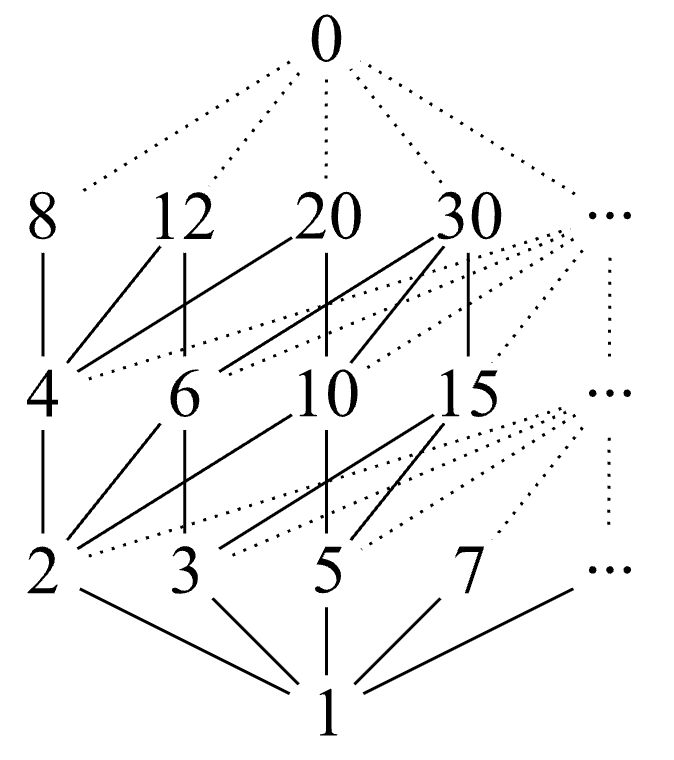
\includegraphics[width=100px]{fig/divisor_lattice.png}
\end{center}

The set $(\mathbb{N}, \preceq)$ forms a preorder. So,
what do products look like in $(\mathbb{N}, \preceq)$ considered 
as a category?
Let's consider the concrete instance of the product of $12$ 
and $16$. Let's consider the three possible interpretations of 
the product of $12$ and $16$ -- let's call it $X$ -- to understand what it means here:\marginnote{In what way 
is this behaving like an intersection?}
\begin{itemize}
  \item The graph-theoretic picture places the product
  in the following diagram for some other object $Y$:
  \item The order theoretic interpretation tells us that 
  $X$ is the greatest element that is less than both $12$
  and $16$ in the partial order -- i.e., it is the 
  greatest lower bound. In the case of this particular 
  partial order, this object has a special name: it is the 
  greatest common divisor.
\end{itemize}



\section{Initial object \& duality}
The categorical picture can push you towards new ideas you may not have thought of.

\section{Products as Terminal Objects ($*$)}
\marginnote{Sections marked with $*$ are optional and won't be covered in class.}

The diagrammatic form suggests a
a order-based intuition for products:
the product \((P,p,q)\) is
in some sense the ``largest''
tuple of that shape,
with its universal property
showing that any other tuple of the same shape is
``less than or equal'' to it by virtue of the existence of
the dashed morphism.

\begin{definition}[category of rooted spans]
  \sloppy
  Let \(A\) and \(B\) be objects of a category \(\calC\).
The category of \emph{spans in \(\calC\) rooted at \(A\) and \(B\)},
written \(\mathsf{Span}_\calC(A,B)\),
is the category whose
\begin{itemize}
  \item Objects are tuples \((X,f,g)\)
    where \(X\) is an object of \(\calC\),
    \(f : X \to A\), and \(g : X \to B\).
    Pictorially:
    \[% https://tikzcd.yichuanshen.de/#N4Igdg9gJgpgziAXAbVABwnAlgFyxMJZABgBoBGAXVJADcBDAGwFcYkQANEAX1PU1z5CKcqWLU6TVuwCCPPiAzY8BIqIBMEhizaIQAIR4SYUAObwioAGYAnCAFskZEDghJ1NbdL2mQNRvQARjCMAAoCKsIgNlimABY48tZ2jojOrkiikjrsVkbcQA
\begin{tikzcd}
                                   & A \\
X \arrow[rd, "g"'] \arrow[ru, "f"] &   \\
                                   & B
\end{tikzcd}\]
  \item A morphism is a tuple
    \(((X,f,g),\alpha,(X',f',g'))\)
    where \((X,f,g)\) and  \((X',f',g')\)
    are objects and \(\alpha : X \to X'\)
    is a morphism of \(\calC\)
    such that \(f' \circ \alpha = f\)
    and \(g' \circ \alpha = g\).
    Pictorially:
    \[% https://tikzcd.yichuanshen.de/#N4Igdg9gJgpgziAXAbVABwnAlgFyxMJZABgBoBGAXVJADcBDAGwFcYkQANEAX1PU1z5CKAEyli1Ok1bsAgjz4gM2PASJiRkhizaIQAIQX8VQouQpbpuzgHIekmFADm8IqABmAJwgBbJGRAcCCQxKR12JxAaRnoAIxhGAAUBVWEQTywnAAscKJB4sCgkAFoAZmJeD28-RACgpHMwmT13PIKixHLKkC9fJFKaesRG7Waeu2i4hOSTNT0M7Nzu3pqBwODEUNHrJztl6v9BjbXt9gAdM6Y0LPp7biA
\begin{tikzcd}
                                                                                &                                       & A \\
X \arrow[rrd, "g"', bend right] \arrow[rru, "f", bend left] \arrow[r, "\alpha"] & X' \arrow[ru, "f'"'] \arrow[rd, "g'"] &   \\
                                                                                &                                       & B
\end{tikzcd}\]

\item Composition is defined by
  \begin{align}
    &((X',f',g'),\alpha',(X'',f'',g''))\circ ((X,f,g),\alpha,(X',f',g'))\\
    &= ((X,f,g),\alpha'\circ \alpha,(X'',f'',g'')).
  \end{align}
  Pictorially:
  \begin{equation}
    % https://tikzcd.yichuanshen.de/#N4Igdg9gJgpgziAXAbVABwnAlgFyxMJZAJgBoAGAXVJADcBDAGwFcYkQBBEAX1PU1z5CKMsWp0mrdgCEefEBmx4CRMgEZxDFm0QgAGgHIDc-kqFE1pDTS1TdhkwoHLhyclc2Sd+493EwoAHN4IlAAMwAnCABbJDIQHAgkdwltdjCjR0iYuJpEpEtUuxBAzJpGegAjGEYABWdzXQisQIALHCyo2MQAZjykxHjbbwAdEaY0VvpfeWzuvoSBlOH04xpqsChk3nCupAX8xEKNrcRlr3ZSkHKqmvqzFSaW9s6cxAAWfuT1mE3987SujCr26n0WBR+f0QAFoegDioFriAKtU6g1HiBmm0OjsQHMkGDDgsVroxhMpjxKNwgA
\begin{tikzcd}
                                                                                 &                                                            & A                                      \\
X' \arrow[rru, "f", bend left] \arrow[rrd, "g"', bend right] \arrow[r, "\alpha"] & X' \arrow[r, "\alpha'"] \arrow[ru, "f'"] \arrow[rd, "g'"'] & X'' \arrow[u, "f''"] \arrow[d, "g''"'] \\
                                                                                 &                                                            & B
\end{tikzcd}
  \end{equation}

  \item The identity morphism at \((X,f,g)\) is \(((X,f,g),\idt_{X},(X,f,g))\).
\end{itemize}
The associativity and identity laws in \(\mathsf{Span}_\calC(A,B)\)
are inherited from the corresponding laws for in \(\calC\).
\end{definition}

This perhaps tortured-looking category serves a valuable purpose:
it makes precise the sense in which a product \((P,p,q)\)
is the ``largest'' among such tuples.

\begin{proposition}
  Let \(A\) and \(B\) be objects of a category \(\calC\).
  A tuple \((P,p,q)\) is a product of \(A\) and \(B\)
  if and only if it is a terminal object of \(\mathsf{Span}_\calC(A,B)\).
\end{proposition}

To unpack what this is saying, from the perspective of categories as metalanguages:
a product for \(A\) and \(B\) in the metalanguage embodied
by \(\calC\) is a unit type for the metalanguage
embodied by \(\mathsf{Span}_\calC(A,B)\).
Some of the power of category theory can be seen here:
\begin{itemize}
\item Constructions on categories can be used to quickly build
  nontrivial ``metalanguages'' from old.
  (What would \(\mathsf{Span}_\calC(A,B)\) even look like as a traditional language?)
\item Category theory ``eats itself'': the categorical notion of terminal object
  sheds light on the categorical notion of product, if one knows to look at
  the right category.
\end{itemize}
To illustrate the benefits of this perspective,
we get a proof that products are suitably unique
just like terminal objects are, simply because they \emph{are terminal objects}:
\begin{proposition}
  Products are unique up to unique isomorphism.
\end{proposition}
\begin{proof}
  Products are terminal objects,
  and terminal objects are unique up to unique isomorphism.
\end{proof}



\chapter{Universal Constructions II}

Let us recall the rules for a language with function types.
First, we have the rule for making terms of function type:
\begin{mathpar}
\inferrule*
    {\Gamma, x \ofty A \vdash M : B}
    {\Gamma \vdash \pllam{x}{M} : A \plto B}
    ~(\textsc{T-Lam})
\end{mathpar}
Next, we have the elimination rule for using terms of function type:
\begin{mathpar}
\inferrule*
    {\Gamma\vdash M : A \plto B
      \\
    \Gamma \vdash N : A
    }
    {\Gamma \vdash \plapp{M}{N} : B}
    ~(\textsc{T-App})
\end{mathpar}
Finally, we have the \(\beta\) and \(\eta\) laws,
which state that applying a function corresponds to
substitution and that every term of function type is equivalent
to a \(\lambda\)-expression.
\begin{mathpar}
\inferrule*
    {
      \Gamma, x\ofty A\vdash M : B
      \\
      \Gamma \vdash N : A
    }
    {\Gamma \vdash \plapp{(\pllam{x}{M})}{N} \equiv M[N/x] : B}
    ~(\beta^{\plto})
\and
\inferrule*
    {\Gamma \vdash M : A \to B}
    {\Gamma \vdash M \equiv \pllam{x}{\plapp{M}{x}} : A \to B}
    ~(\eta^{\plto})
\end{mathpar}

In category theory, this language feature is captured by
the concept of an \emph{exponential object}.
\newcommand\app{\mathsf{app}}
\newcommand\lam{\lambda}
\begin{definition}
  \sloppy
  Let \(X\) and \(Y\) be objects of a category \(\calC\) with products.
  An \emph{exponential of \(X\) by \(Y\)}
  is a pair \((E,\app)\) consisting of
  an object \(E\) of \(\calC\)
  and a morphism
  \(\app : E\times X \to Y\)
  such that the following universal property holds:
  for all morphisms \(f : \Gamma \times X \to Y\),
  there exists a unique morphism \(\lam f : \Gamma \to E\)
  such that \(\app \circ \angled{\lam f \circ \pi_1, \pi_2} = f\).
\end{definition}

Note that the morphism \(\app\)
has a domain defined by a product,
and the universal property of \((E,\app)\)
is stated in terms of the morphism \(\angled{\lam f \circ \pi_1,\pi_2}\),
whose existence depends on the existence of products.
In this way, the definition of exponential objects
requires products in \(\calC\) as a prerequisite.%
\footnote{There are actually tricks to define
the notion of ``function object'' categorically
without reference to products, but that will have to wait until after Yoneda IV.}

\noindent How does this definition capture the familiar rules for function types?
\begin{itemize}
  \item The object \(E\) models the function space \(X \to Y\).
  \item \(\app\) corresponds to function application:
    \(f\ofty E, x\ofty X \vdash f\plapp x : Y\).
  \item The universal property models \textsc{T-Lam}.
  \item What to make of the equation \(\app \circ \angled{\lam f \circ \pi_1, \pi_2} = f\)?
\end{itemize}

\noindent To understand, we need to take a slightly more detailed look at how to
    translate terms into categorical combinators.
\begin{itemize}
  \item Recap of products: each term formation rule becomes an operation on morphisms.
    Typing derivations can be translated into categorical combinators this way.
    Example: fst (x, y)
  \item Each equational law becomes an equality of composites.
    Example: fst (x, y) = x.
  \item Subtle point: weakening as precomposition by structural maps.
    Example: suppose M is well typed under Gamma; interpret M under Gamma,x:A.
\end{itemize}

Armed with this knowledge, let's try and backtranslate
    \(\app \circ \angled{\lam f \circ \pi_1, \pi_2} = f\)
    into familiar language.
\todo

\begin{itemize}
  \item Recall the three perspectives:
    \begin{itemize}
    \item Algebraic: beta and eta rules as equations
    \item Graphical: the triangle commutes
    \item Order-theoretic: exponential as largest code pointer (formally:
            terminal in a category of code pointers)
    \end{itemize}
\end{itemize}
\todo

\begin{itemize}
  \item Examples
    \begin{itemize}
    \item Exponentials in FinSet are function spaces
    \item Exponentials in open subsets of the plane are a funny thing (remember:
      largest code pointer)
    \end{itemize}
\end{itemize}
\todo

\begin{itemize}
  \item What's really going on? Brief interlude: getting formal about categorical semantics
\end{itemize}
Wellformedness rules
\[
s ::= (M,\dots)
\]
\[
\fbox{\(s : \Gamma \longrightarrow \Gamma'\)}
\]
\begin{mathpar}
\inferrule
    {\Gamma \vdash M : A
      \\\dots}
    {(M,\dots) : \Gamma \longrightarrow x\ofty A,\dots}
\end{mathpar}
The following rule is admissible:
\begin{mathpar}
  \inferrule{\Gamma \vdash M : A \\ s : \Gamma'\longrightarrow\Gamma}
            {\Gamma' \vdash M[s] : A}
\end{mathpar}
Semantically,
\[
\text{if \(s : \Gamma\longrightarrow\Gamma'\)
then \(\llbr{s} : \llbr{\Gamma} \to \llbr{\Gamma'}\)}
\]
\footnote{The dreaded ``substitution lemma'' that all mechanizers hate}
\[
\llbr{M[s]} = \llbr{M} \circ \llbr{s}
\]
All semantic interpretation functions must be stable
under substitution/precomposition:
\begin{align*}
  \plpair{M}{N}[s] &= \plpair{M[s]}{N[s]}
  &
  \angled{f,g} \circ p &= \angled{f\circ p,g\circ p}
  \\
  \plfst{M}[s] &= \plfst{M[s]}
  &
  (\pi_1 \circ f) \circ p &= \pi_1 \circ (f \circ p)
\end{align*}

\begin{itemize}
  \item Distributivity, ``high school algebra laws''
\end{itemize}
\todo

%%%%%%%%%%%%%%%%%%%%%%%%%%%%%%%%%%%%%%%%%%%%%%%%%%%%%%%%%%%%%%%%%%%%%%%%%%%%%%%%
%%%%%%%%%%%%%%%%%%%%%%%%%%%%%%%%%%%%%%%%%%%%%%%%%%%%%%%%%%%%%%%%%%%%%%%%%%%%%%%%


% - Give standard rules for function types
% - Golf rules using substitution
% - Reverse engineer textbook definition
